\documentclass{beamer}

\usepackage[frenchb]{babel}
\usepackage[utf8]{inputenc}
\usepackage{default}

\usetheme{Luebeck}
%\setbeamercolor*{palette primary}{use=structure,fg=white,bg=gray}
%\setbeamercolor*{palette quaternary}{fg=white,bg=black}

\title[Présentation de 7Robot 2013-2014]{Présentation de 7Robot 2013-2014\\ Le club et ses activités}
\author{7Robot}
\date{\today}

\setbeamertemplate{navigation symbols}{
  \insertframenavigationsymbol % Icône slide
  \insertbackfindforwardnavigationsymbol % Icône backfindforward
}
\setbeamertemplate{background canvas}{\includegraphics[width=\paperwidth,height=\paperheight]{../images/fond.png}}

\AtBeginSection[]{
  \begin{frame}
  \tableofcontents[currentsection, hideothersubsections]
  \end{frame} 
}

\begin{document}

\begin{frame}
  \titlepage
\end{frame}

\begin{frame}
  \tableofcontents
\end{frame}

\section{Le club 7Robot}
  \begin{frame}
   \begin{itemize}
      \item Le club de robotique de l'ENSEEIHT
      \item Un local (salle E117) avec du matériel
      \item De nombreux membres (plus de 1 c'est nombreux hein ? \^{}\^{})
      \item Des projets variés (coupe de France, coupe Freescale ...)
   \end{itemize}

   \begin{center}
      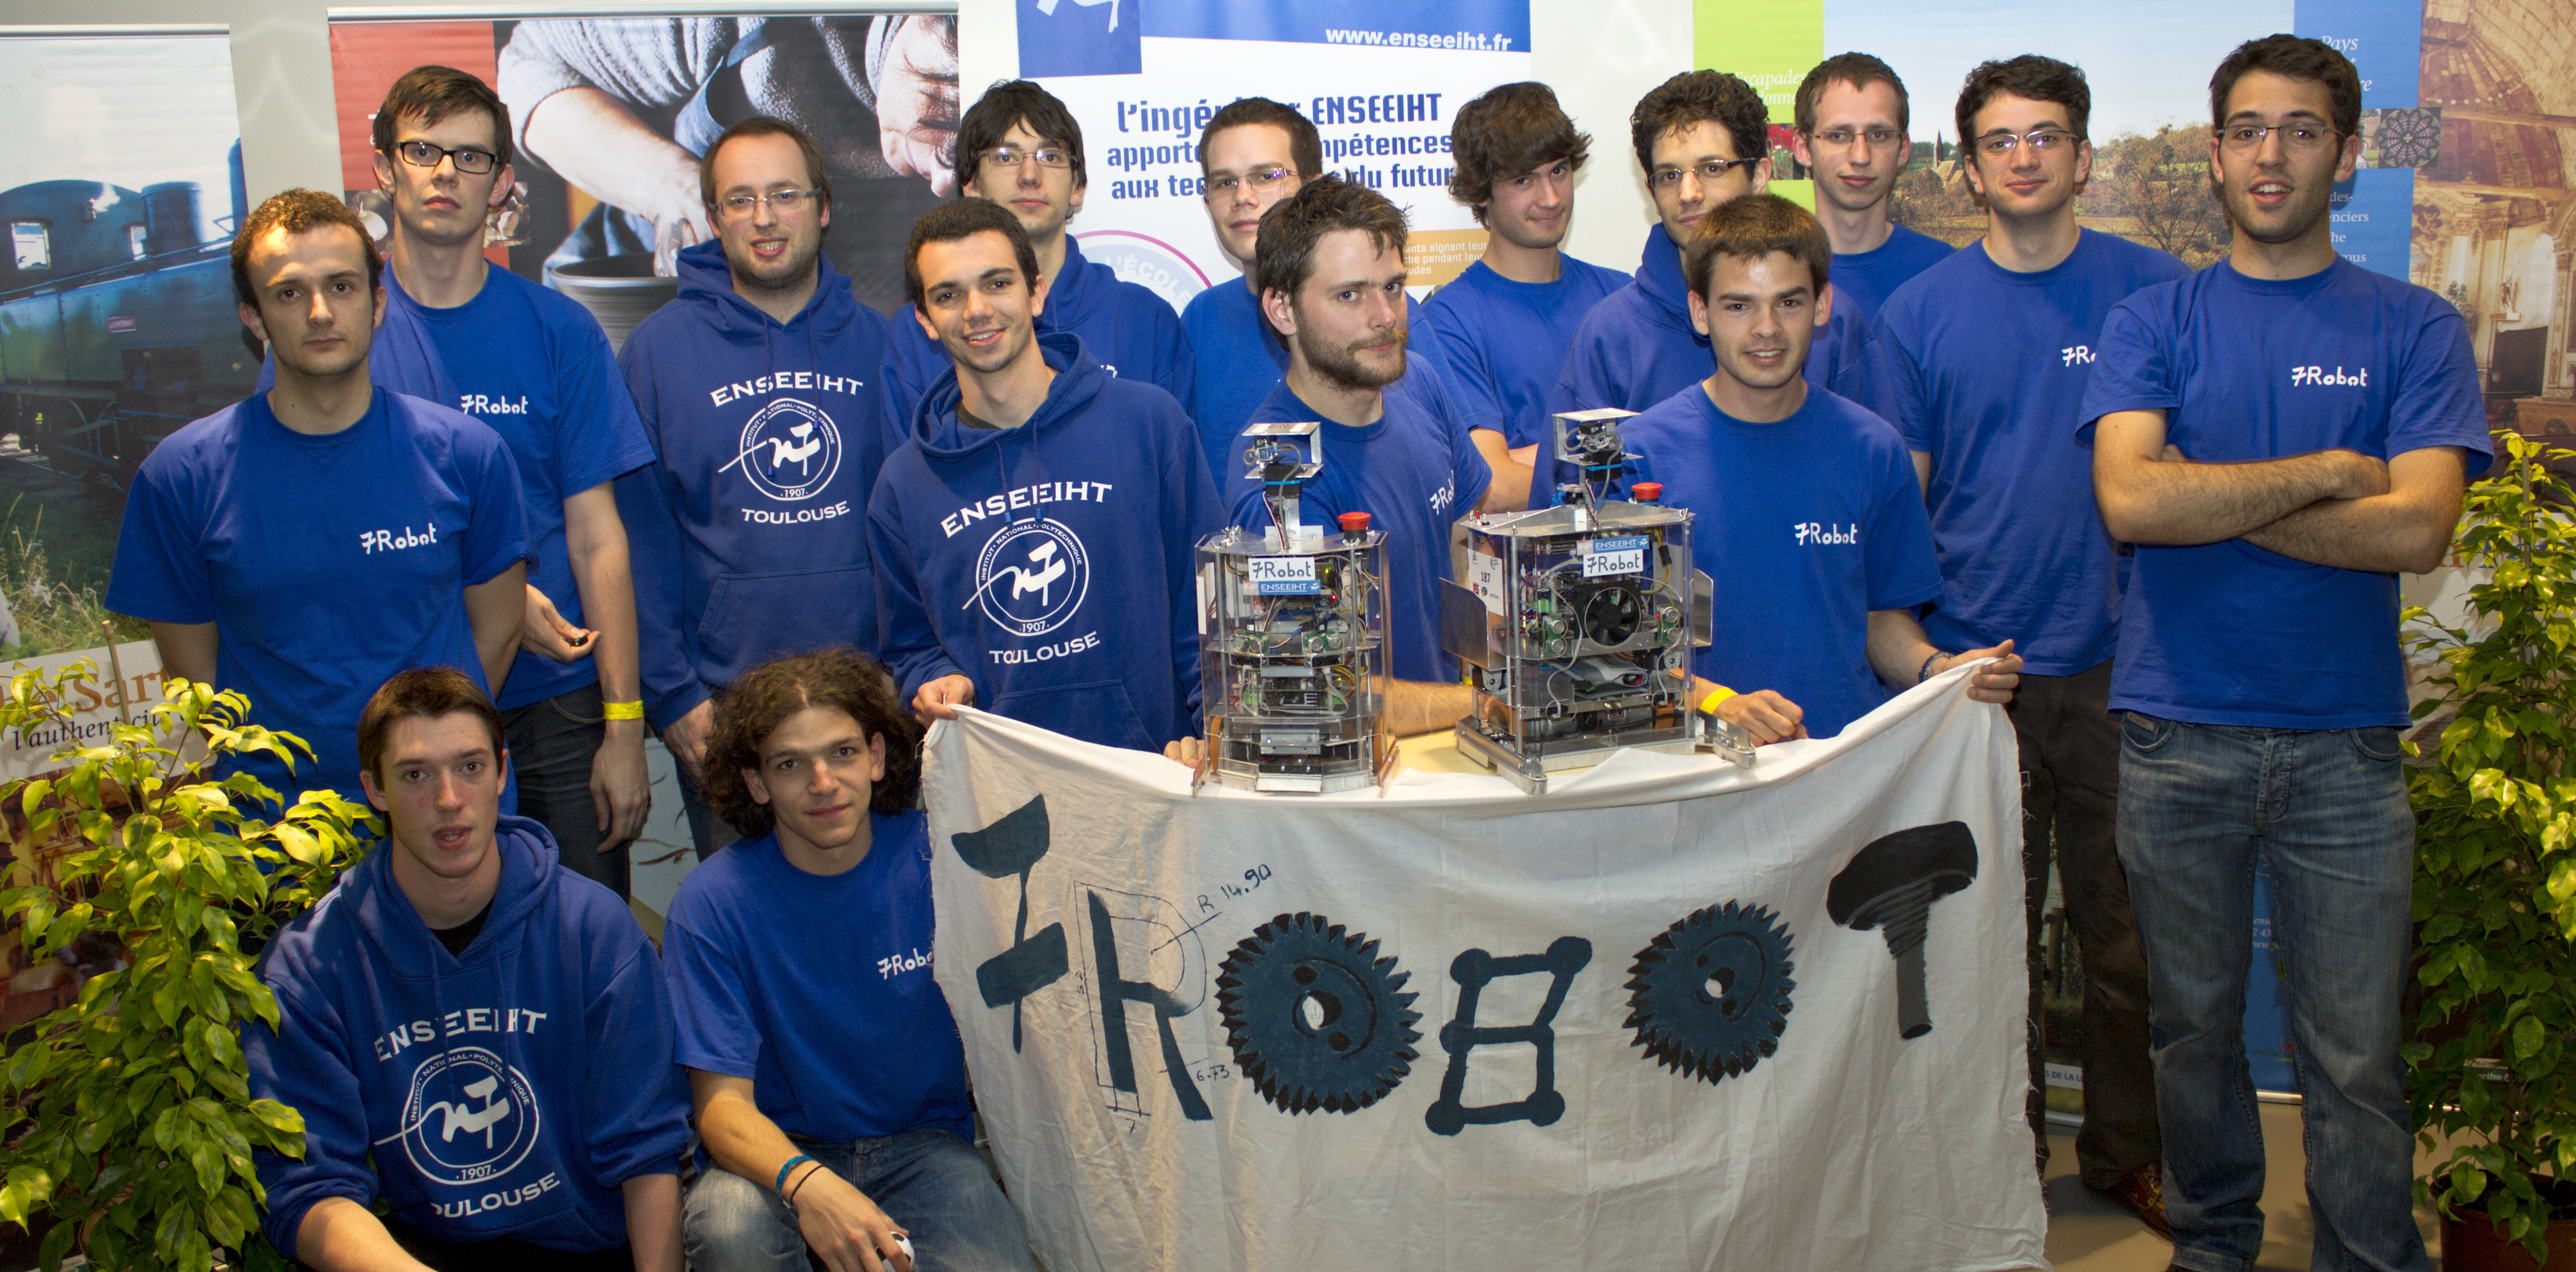
\includegraphics[width=0.8\textwidth]{../images/groupe.jpg}
   \end{center}
\end{frame}

\begin{frame}
Bureau 2012-2013 :\\
   \begin{tabular}{rl}
      Président : & Ken Hasselmann \\
      Vice-Président : & Elie Bouttier \\
      Trésorier : & Guillaume Dib \\
      Secrétaire : & Thomas Nicot \\
   \end{tabular}

\vspace{1em}
Bureau 2013-2014 :\\
   \begin{tabular}{rl}
      Président : & Matthieu Pizenberg \\
      Trésorier : & Korantin Auguste \\
      Secrétaire : & Antoine Hochenedel \\
   \end{tabular}
\end{frame}


\section{Les activités du club}
  \subsection{Coupe de France de Robotique}
    \begin{frame}
   \begin{center}
      \includegraphics[width=0.7\textwidth]{../images/cdf.jpg}
   \end{center}
   \begin{itemize}
      \item une coupe internationnalle (Eurobot)
      \item près de 200 équipes (écoles, universités, associations ...)
      \item des rencontres, une super ambiance, des nuits blanches ...
   \end{itemize}
\end{frame}

\begin{frame}
   \begin{center}
      \movie[externalviewer]{\includegraphics[width=\textwidth]{../images/cdf2013.png}}{../videos/test.avi}
   \end{center}
\end{frame}

  \subsection{Coupe Freescale}
    \begin{frame}
Course de voitures miniatures automatiques.
Circuit constitué d'une ligne noire : faire un tour le plus vite possible.

Qualifications française organisée à l'N7 cette année.

\begin{block}{Résultats}
    2è, qualifiés pour la finale européenne en Allemagne.
\end{block}

\end{frame}

  \subsection{Autres activités}
    \begin{frame}
   \begin{itemize}
      \item La semaine de bar
      \item Vos projets en tout genre
   \end{itemize}
\end{frame}


\section{Coupe de France 2014}
  \input{cdf2014.tex}
  
\section{Formations}
  \begin{frame}
   \begin{itemize}
      \item Formation Git :
      \item Formation Arduino (et C) :
   \end{itemize}
\end{frame}


\end{document}
